\documentclass[a4paper,14pt]{extreport}
\usepackage[left=1.5cm,right=1.5cm,
    top=1.5cm,bottom=2cm,bindingoffset=0cm]{geometry}
\usepackage{scrextend}
\usepackage[T1,T2A]{fontenc}
\usepackage[utf8]{inputenc}
\usepackage[english,russian,ukrainian]{babel}
\usepackage{tabularx}
\usepackage{amssymb}
\usepackage{color}
\usepackage{amsmath}
\usepackage{mathrsfs}
\usepackage{listings}
\usepackage{graphicx}
\graphicspath{ {./images/} }
\usepackage{lipsum}
\usepackage{xcolor}
\usepackage{hyperref}
\usepackage{tcolorbox}
\usepackage{tikz}
\usepackage[framemethod=TikZ]{mdframed}
\usepackage{wrapfig,boxedminipage,lipsum}
\mdfdefinestyle{MyFrame}{%
linecolor=blue,outerlinewidth=2pt,roundcorner=20pt,innertopmargin=\baselineskip,innerbottommargin=\baselineskip,innerrightmargin=20pt,innerleftmargin=20pt,backgroundcolor=gray!50!white}
 \usepackage{csvsimple}
 \usepackage{supertabular}
\usepackage{pdflscape}
\usepackage{fancyvrb}
%\usepackage{comment}
\usepackage{array,tabularx}
\usepackage{colortbl}

\usepackage{varwidth}
\tcbuselibrary{skins}
\usepackage{fancybox}


\usepackage{tikz}
\usepackage[framemethod=TikZ]{mdframed}
\usepackage{xcolor}
\usetikzlibrary{calc}
\makeatletter
\newlength{\mylength}
\xdef\CircleFactor{1.1}
\setlength\mylength{\dimexpr\f@size pt}
\newsavebox{\mybox}
\newcommand*\circled[2][draw=blue]{\savebox\mybox{\vbox{\vphantom{WL1/}#1}}\setlength\mylength{\dimexpr\CircleFactor\dimexpr\ht\mybox+\dp\mybox\relax\relax}\tikzset{mystyle/.style={circle,#1,minimum height={\mylength}}}
\tikz[baseline=(char.base)]
\node[mystyle] (char) {#2};}
\makeatother

\definecolor{ggreen}{rgb}{0.4,1,0}
\definecolor{rred}{rgb}{1,0.1,0.1}
\definecolor{amber}{rgb}{1.0, 0.75, 0.0}
\definecolor{babyblue}{rgb}{0.54, 0.81, 0.94}
\definecolor{amethyst}{rgb}{0.6, 0.4, 0.8}
\usepackage{graphicx}
\usepackage{float}
\usepackage{wrapfig}
\usepackage{framed}
%for nice Code{
\lstdefinestyle{customc}{
  belowcaptionskip=1\baselineskip,
  breaklines=true,
  frame=L,
  xleftmargin=\parindent,
  language=C,
  showstringspaces=false,
  basicstyle=\small\ttfamily,
  keywordstyle=\bfseries\color{green!40!black},
  commentstyle=\itshape\color{purple!40!black},
  identifierstyle=\color{blue},
  stringstyle=\color{orange},
}
\lstset{escapechar=@,style=customc}
%}


\begin{document}
\pagecolor{white}

%----------------------------------------1
\newtcbox{\xmybox}[1][red]{on line, arc=7pt,colback=#1!10!white,colframe=#1!50!black, before upper={\rule[-3pt]{0pt}{10pt}},boxrule=1pt, boxsep=0pt,left=6pt,right=6pt,top=2pt,bottom=2pt}

\begin{titlepage}
  \begin{center}
    \large
    Національний технічний університет України \\ "Київський політехнічний інститут імені Ігоря Сікорського"


    Факультет Електроніки

    Кафедра мікроелектроніки
    \vfill

    \textsc{ЗВІТ}\\

    {\Large Про виконання курсової роботи \\
      з дисципліни: «Твердотільна електроніка-2»\\[1cm]

        Варіант №50


    }
  \bigskip
\end{center}
\vfill

\newlength{\ML}
\settowidth{\ML}{«\underline{\hspace{0.4cm}}» \underline{\hspace{2cm}}}
\hfill
\begin{minipage}{1\textwidth}
Виконавець:\\
Студент 3-го курсу \hspace{4cm} $\underset{\text{(підпис)}}{\underline{\hspace{0.2\textwidth}}}$  \hspace{1cm}А.\,С.~Мнацаканов\\
\vspace{1cm}

Перевірив: \hspace{6.1cm} $\underset{\text{(підпис)}}{\underline{\hspace{0.2\textwidth}}}$  \hspace{1cm}Л.\,М.~Королевич\\

\end{minipage}

\vfill

\begin{center}
2021
\end{center}
\end{titlepage}

\begin{center}
    \textbf{Завдання}
\end{center}
Побудувати креслення схеми електричної
Проаналізувати роботу схеми:

\begin{enumerate}
  \item Розробити схему електричну принципову мікросхеми на основі прототипу вказаного за варіантом
  \item Побудувати таблицю істинності та визначити логічну функцію, яку виконує мікросхема.
  \item побудувати логічну функцію (схема)
\end{enumerate}

\begin{center}
  \textbf{Виконання завдання}
\end{center}

\begin{figure}[h!]
\center{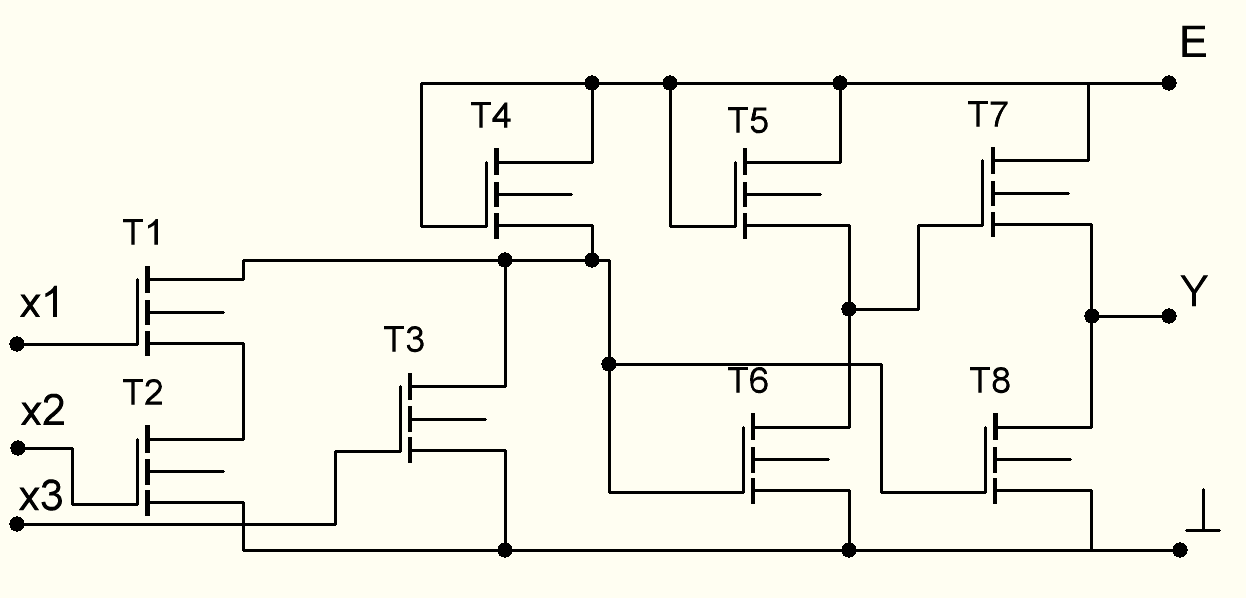
\includegraphics[width=1\linewidth]{1-a.png}}
\caption{Прототип схеми.}
\label{ris1}
\end{figure}
У мене за варіантом тип підкладки КЕФ, тобто n-тип підкладки, тоді $Rightarrow$ p-канал у транзисторах.

\begin{figure}[h!]
\center{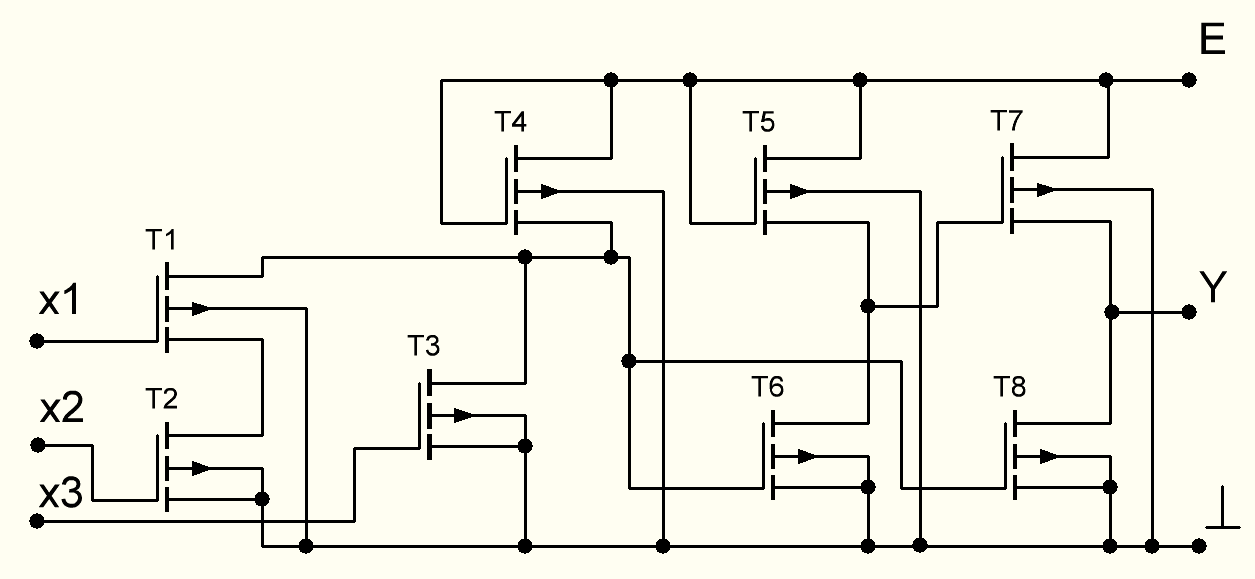
\includegraphics[width=1\linewidth]{2-a.png}}
\caption{Електрична схема на основі прототипу.}
\label{ris2}
\end{figure}
Оскільки у нас інтегральна мікросхема, то треба аби всі підкладки були підключені до спільного вивод, що і показано на рис.\ref{ris2}.\\

Тепер переходимо до наступного завдання. Треба скласти таблицю істинності, але легше зробити це розбивши схему на каскади. Розглядати будемо спрощену модель схеми (бо так простіше), замінивши усі транзистори змінними резисторами, окрім T4 і T5. Так як у них затвор під’єднаний до стоку, то ці транзистори будуть грати роль нагрузки, тобто заміняємо їх звичайними резисторами.
\newpage


\begin{figure}[h!]
\begin{center}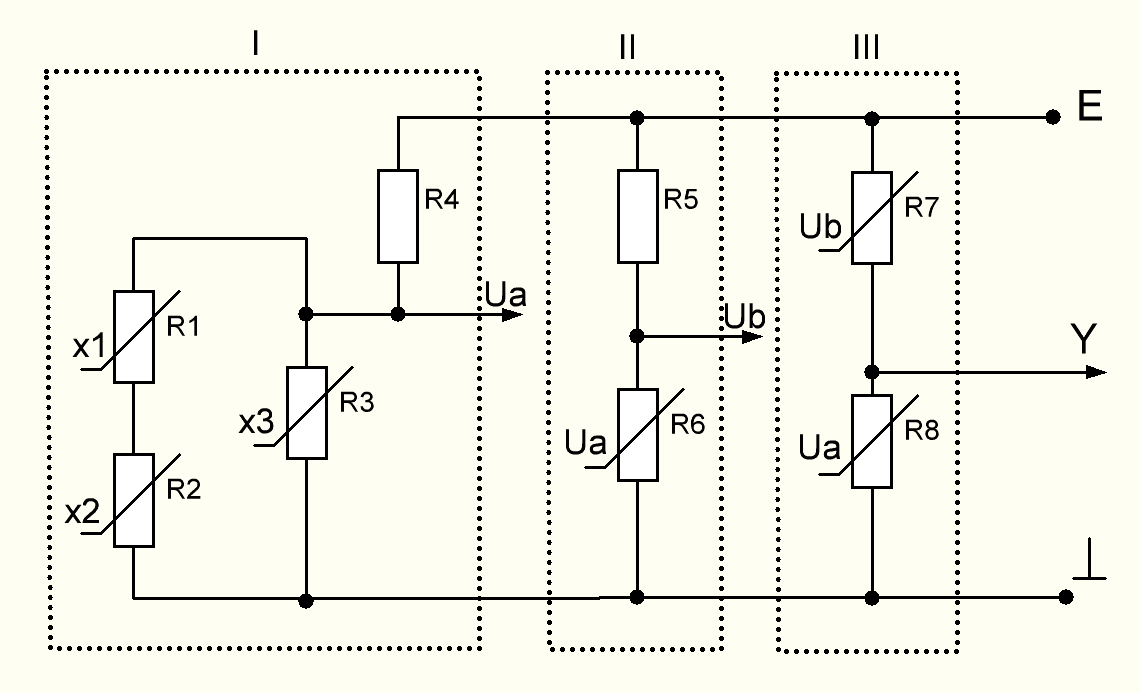
\includegraphics[width=1\linewidth]{3-a.png}\end{center}
\caption{Спрощена модель.}
\label{ris3}
\end{figure}


Бачимо, що у цій схемі всього три каскади. Розпочнемо з першого. У нас три змінних резистори, які можна об’єднати в один (спочатку R1 I R2, так як вони послідовно з'єднані, і потім з R3, так як паралельно підключені). Покроково це виглядатиме так:


\newpage

\begin{figure}[h!]
\center{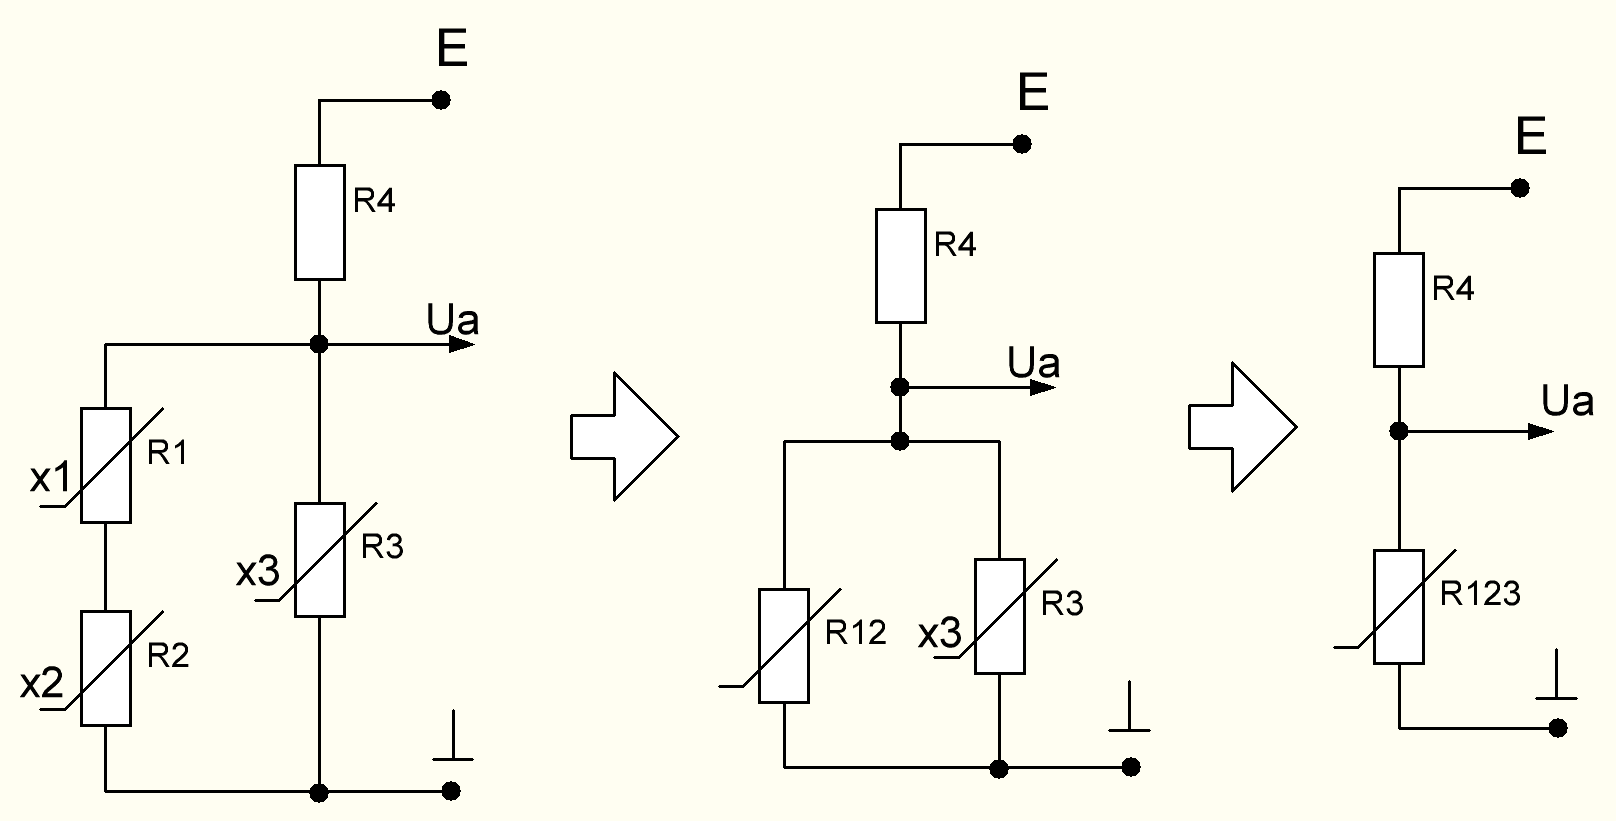
\includegraphics[width=1\linewidth]{4-a.png}}
\label{ris4}
\end{figure}

\begin{align}
  R_{12} = R_1 + R_2
\end{align}
\begin{align}
  R_{123} = \dfrac{R_{12} \cdot R_3}{R_{12} + R_3} = \dfrac{R_{1}+R_{2} \cdot R_3}{R_{1}+R_{2} + R_3}
\end{align}

По нашому скороченню, у нас вийшов резистивний дільник напруги (по резисторам $R_{4}$ i $R_{123}$). Знаходимо напругу $U_a$.

\begin{align}
  U_a = \dfrac{R_{123} \cdot E}{R_{4} + R_{123}}
\end{align}
По цих формулах уже можемо складати таблицю істинності для першого каскаду. Аби було легше рахувати, приймемо, що $R_{3} \rightarrow 0$ , а потім, що $R_{3} \rightarrow \infty$.

\begin{table}[h]
  \begin{center}
    \begin{tabular}{|c|c|c|c|c|}
    \hline
    $R_1 $  & 1 & 1 & 0 & 0 \\ \hline
    $R_2 $  & 1 & 0 & 1 & 0 \\ \hline
    $R_3 $  & 0 & 0 & 0 & 0 \\ \hline
    $R_{123} $& 0 & 0 & 0 & 0 \\ \hline
    $U_a  $ & 0 & 0 & 0 & 0 \\ \hline
    \end{tabular}
  \end{center}
\end{table}
Тепер для $R_{3} \rightarrow \infty$













\begin{align}
R_{123}=\frac{\left(R_{1}+R_{2}\right) \cdot R_{3}}{R_{3} \frac{\left(R_{1}+R_{2}\right)}{R_{3}}+R_{3}}=\frac{\left(R_{1}+R_{2}\right) \cdot R_{3}}{R_{3}\left(\frac{\left(R_{1}+R_{2}\right)}{R_{3}}+1\right)}=
 \frac{\left(R_{1}+R_{2}\right)}{\left(\frac{\left(R_{1}+R_{2}\right)}{R_{3}}+1\right)}=\frac{\left(R_{1}+R_{2}\right)}{(0+1)}=R_{1}+R_{2}
\end{align}



\begin{table}[h]
  \begin{center}
    \begin{tabular}{|c|c|c|c|c|}
    \hline
    R1   & 1 & 1 & 0 & 0 \\ \hline
    R2   & 1 & 0 & 1 & 0 \\ \hline
    R3   & 1 & 1 & 1 & 1 \\ \hline
    R123 & 1 & 1 & 1 & 0 \\ \hline
    Ua   & 1 & 1 & 1 & 0 \\ \hline
    \end{tabular}
  \end{center}
\end{table}



Тоді, загальна таблиця разом з x1, x2, x3 матиме вигляд:


\begin{table}[h]
  \begin{center}
    \begin{tabular}{|c|c|c|c|c|c|c|c|c|}
    \hline
    X1   & 0 & 0 & 0 & 0 & 1 & 1 & 1 & 1 \\ \hline
    X2   & 0 & 1 & 0 & 1 & 0 & 1 & 0 & 1 \\ \hline
    X3   & 0 & 0 & 1 & 1 & 0 & 0 & 1 & 1 \\ \hline
    R1   & 1 & 1 & 1 & 1 & 0 & 0 & 0 & 0 \\ \hline
    R2   & 1 & 0 & 1 & 0 & 1 & 0 & 1 & 0 \\ \hline
    R3   & 1 & 1 & 0 & 0 & 1 & 1 & 0 & 0 \\ \hline
    R123 & 1 & 1 & 0 & 0 & 1 & 0 & 0 & 0 \\ \hline
    Ua   & 1 & 1 & 0 & 0 & 1 & 0 & 0 & 0 \\ \hline
    \end{tabular}
  \end{center}
\end{table}


Усе, таблиця істинності 1 каскаду зроблена. Далі переходимо до 2 і 3 каскаду:




\begin{figure}[h!]
\center{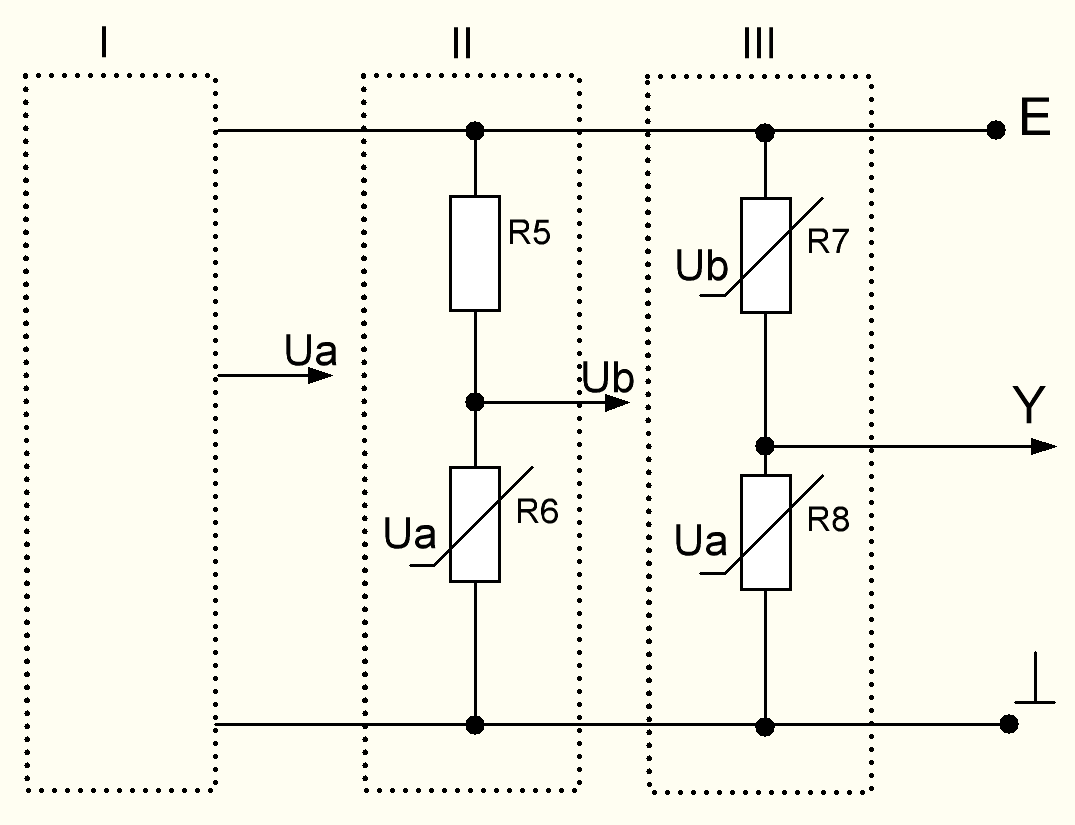
\includegraphics[width=0.7\linewidth]{5-a.png}}
\label{ris5}
\end{figure}
Тут два дільники напруги. Можемо одразу скласти формули напруги для Ub та Y:
\begin{equation}
U_{b}=\frac{R_{6}}{R_{5}+R_{6}} \cdot E \quad Y=\frac{R_{8}}{R_{7}+R_{8}} \cdot E
\end{equation}

Складаємо таблицю істинності одразу для двох каскадів:

\begin{table}[h]
  \begin{center}
  \begin{tabular}{|c|c|c|}
  \hline
  Ua & 1 & 0 \\ \hline
  R6 & 0 & 1 \\ \hline
  Ub & 0 & 1 \\ \hline
  R7 & 1 & 0 \\ \hline
  R8 & 0 & 1 \\ \hline
  Y  & 0 & 1 \\ \hline
  \end{tabular}
  \end{center}
\end{table}

Таблиця істинності 2 і 3 каскаду є. Тепер об’єднаємо таблиці істинності першого і другого – третього каскадів:


\begin{table}[h]
  \begin{center}
\begin{tabular}{|c|c|c|c|c|c|c|c|c|}
\hline
X1 & 0 & 0 & 0 & 0 & 1 & 1 & 1 & 1 \\ \hline
X2 & 0 & 1 & 0 & 1 & 0 & 1 & 0 & 1 \\ \hline
X3 & 0 & 0 & 1 & 1 & 0 & 0 & 1 & 1 \\ \hline
Ua & 1 & 1 & 0 & 0 & 1 & 0 & 0 & 0 \\ \hline
Ub & 0 & 0 & 1 & 1 & 0 & 1 & 1 & 1 \\ \hline
Y  & 0 & 0 & 1 & 1 & 0 & 1 & 1 & 1 \\ \hline
\end{tabular}
  \end{center}
\end{table}

Ми побачили, що другий каскад інвертуючий, через що Ub має протилежні знаки відносно Ua, а третій каскад не є інвертуючим, тому і має те саме, що Ub.
Далі складаємо логічну функцію по отриманій таблиці:
\begin{equation}
\begin{array}{l}
Y=\bar{x}_{1} \cdot \bar{x}_{2} \cdot x_{3}+\bar{x}_{1} \cdot x_{2} \cdot x_{3}+x_{1} \cdot x_{2} \cdot \bar{x}_{3}+x_{1} \cdot \bar{x}_{2} \cdot x_{3}+x_{1} \cdot x_{2} \cdot x_{3}= \\
=\bar{x}_{1} \cdot x_{3}++x_{1} \cdot x_{2} \cdot \bar{x}_{3}+x_{1} \cdot x_{3}=x_{3}+x_{1} \cdot x_{2} \cdot \bar{x}_{3}=x_{3}+x_{1} \cdot x_{2}
\end{array}
\end{equation}



І далі, останній крок, малюємо логічну схему по формулі:


\begin{figure}[h!]
\center{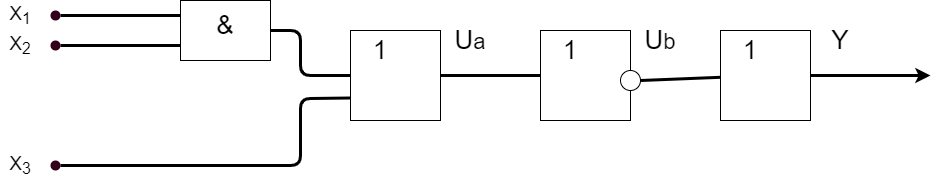
\includegraphics[width=0.9\linewidth]{courseW-a.png}}
\label{ris6}
\end{figure}


















\end{document}
